% ============================================================
% Open VCV Paper — LaTeX source
% Compile: pdflatex paper.tex && pdflatex paper.tex
% ============================================================
\documentclass[10pt,twocolumn]{article}

\usepackage[margin=1in]{geometry}
\usepackage{amsmath,amssymb,amsfonts}
\usepackage{graphicx}
\usepackage{booktabs}
\usepackage{hyperref}
\usepackage{microtype}
\usepackage{xcolor}
\usepackage{enumitem}
\usepackage{caption}
\usepackage{subcaption}
\usepackage{algorithm}
\usepackage{algpseudocode}
\usepackage{listings}
\usepackage{tikz}
\usetikzlibrary{arrows.meta, positioning, shapes.geometric, fit, backgrounds}

% ---- Code style ----
\lstset{
  basicstyle=\ttfamily\footnotesize,
  breaklines=true,
  frame=single,
  backgroundcolor=\color{gray!8},
  keywordstyle=\color{blue!70!black},
  commentstyle=\color{green!50!black},
}

% ---- Title ----
\title{\textbf{Open VCV: Augmentation-Aware Intersect-Union Decomposition\\
via Efficient Gated Residual Encoding}\\[0.5em]
{\normalsize Draft v0.3 --- May 13, 2026}}

\author{Anonymous Submission}
\date{}

% ============================================================
\begin{document}
\maketitle

% ============================================================
\begin{abstract}
We present \textbf{Open VCV} (Open Visual Concept Vocabulary), a self-supervised
visual representation framework that decomposes image features into two orthogonal
components: an \emph{intersection vector} capturing augmentation-invariant semantics,
and a \emph{unique vector} encoding augmentation-specific appearance.

Our core architectural contribution is the \textbf{Fused Gated Multi-Head Convolution
(FGMC)}, which consolidates three independent convolutional operations into a single
kernel call, reducing CUDA kernel launches from 3 to 1 and yielding up to $1.18\times$
wall-clock speedup at deeper layers. We further propose \textbf{Hard Latent Partitioning
(HLP)}, which enforces strict decomposition by directly slicing the VAE latent mean
$\mu$, preventing the feature collapse observed in projection-head architectures. On
the efficiency front, combining AMP, gradient checkpointing, and NHWC memory layout
enables training with latent dimension $D{=}2048$ at batch 64 on a 12\,GB GPU with
only 7.17M parameters---a $3.95\times$ parameter reduction over ResNet-50. An
\textbf{Augmentation-Aware Dynamic Weighting} (AADW) mechanism adaptively scales
loss contributions based on the visual distance between augmented views, yielding
measurably better decomposition than fixed-weight baselines.

\emph{Status note (May 13, 2026).} The experiments reported here cover 5 epochs of
training on COCO 2017 with the baseline encoder architecture plus 1 epoch with the
refactored FGMC backbone. Full 20-epoch training is in progress. Section~\ref{sec:results}
presents current partial results alongside zero-shot baseline comparisons.
\end{abstract}

% ============================================================
\section{Introduction}
\label{sec:intro}

Self-supervised visual learning has advanced rapidly through contrastive
frameworks~\cite{simclr,moco,byol}. These methods share a core design principle:
treat all augmented views of an image as equivalent positive pairs and maximize
their agreement, discarding all view-specific information by construction.

Consider two augmented views of the same photograph: one with heavy color jitter
and one with an aggressive spatial crop. A model mapping both to the same
representation has learned neither the color statistics nor the spatial
relationship---only the semantic category. For downstream tasks such as image
editing, style transfer, or dense prediction, this loss is fundamental.

We formalize the desired decomposition:

\begin{quote}
\textbf{Definition (Intersect-Union Decomposition).} Given an image $x$ with
augmented views $\{x_1,\ldots,x_q\}$, learn encoder $f\!: x \mapsto
(\mathbf{v}_{\rm inter}, \mathbf{v}_{\rm unique})$ such that: (i) \emph{Union
invariance}---$\mathbf{v}_{\rm inter}(x_i)\approx \mathbf{v}_{\rm inter}(x_j)$
for all $i,j$; (ii) \emph{Unique equivariance}---$\mathbf{v}_{\rm unique}(x_i)
\not\approx \mathbf{v}_{\rm unique}(x_j)$ when aug-distance is large; (iii)
\emph{Orthogonality}---$\langle \mathbf{v}_{\rm inter}, \mathbf{v}_{\rm unique}
\rangle \approx 0$.
\end{quote}

\paragraph{Contributions.}
\begin{enumerate}[leftmargin=*, nosep]
\item \textbf{FGMC}: Fused Gated Multi-Head Convolution reduces CUDA kernel
launches from 3 to 1, yielding $1.05$--$1.18\times$ wall-clock speedup at
intermediate and deep layers (batch=64, RTX 3060 12\,GB).
\item \textbf{HLP}: Hard Latent Partitioning enforces gradient isolation between
$\mathbf{v}_{\rm inter}$ and $\mathbf{v}_{\rm unique}$ via direct $\mu$-slicing,
eliminating projection-head collapse.
\item \textbf{AADW}: Augmentation-Aware Dynamic Weighting computes loss weights
$w_{ij}{=}\cos(\mathbf{f}_i, \mathbf{f}_j)$ from intermediate image features,
adapting alignment/divergence pressure to actual visual distance.
\item \textbf{Efficient stack}: AMP + per-stage gradient checkpointing + NHWC +
FGMC enables $D{=}2048$, batch 64 on 12\,GB VRAM at 7.17M parameters, training
at $\approx$563\,imgs/s (backbone inference) on an RTX 3060.
\end{enumerate}

% ============================================================
\section{Related Work}
\label{sec:related}

\paragraph{Contrastive SSL.}
SimCLR~\cite{simclr} maximizes NT-Xent between positive pairs via a projection
head. MoCo~\cite{moco} uses a momentum encoder and queue. BYOL~\cite{byol}
eliminates negatives with an asymmetric predictor. Barlow Twins~\cite{barlow}
decorrelates representations via cross-correlation. VICReg~\cite{vicreg} adds
explicit variance and covariance terms. \emph{All methods produce a single
invariant representation; we produce two complementary ones.}

\paragraph{Equivariant and disentangled representations.}
Ada-GVAE~\cite{adagvae} identifies changing factors across views via discrete
masks. AugSelf~\cite{augself} predicts augmentation parameters as an auxiliary
objective. iDML~\cite{idml} decomposes into class-shared and instance-specific
parts. \emph{We do not predict augmentation parameters nor require supervision.}

\paragraph{Gated convolutions.}
DeepFill~\cite{deepfill} applies gated convolution to inpainting. Our FGMC
adapts gating as an efficient multi-head extractor, replacing three kernels with one
fused operation.

\paragraph{Efficient training.}
Gradient checkpointing~\cite{gradckpt} trades recomputation for memory. AMP
\cite{amp} halves memory bandwidth. NHWC layout improves tensor core
utilization. We combine all three in a principled stack.

% ============================================================
\section{Method}
\label{sec:method}

\subsection{Data Pipeline}

For each step, $B$ images are sampled. Each image $x$ generates $q{=}3$
augmented views: conservative (flip, mild crop), moderate (color jitter,
rotation), and aggressive (cutout, solarize). Additionally, $k{=}2$ independent
negative images $\{n_1,n_2\}$ are sampled from the same batch.

\subsection{Fused Gated Multi-Head Convolution}

\paragraph{Naive formulation (3 launches).}
\begin{equation}
\mathrm{out} = \mathrm{LReLU}\!\bigl(f_\theta(x)\cdot g_\phi(x) + b_\psi(x)\bigr)
\label{eq:naive}
\end{equation}
where $f_\theta, g_\phi, b_\psi \in \mathrm{Conv2d}(C_{\rm in}, C_{\rm out}, 3)$
each dispatch a separate CUDA kernel.

\paragraph{Fused formulation (1 launch).}
\begin{align}
[\mathbf{F}, \mathbf{G}, \mathbf{B}] &= W_{\rm fused} * x,
  \quad W_{\rm fused} \in \mathbb{R}^{3C_{\rm out} \times C_{\rm in} \times 3 \times 3}
  \label{eq:fused_conv} \\
\mathrm{out} &= \mathrm{LReLU}\!\bigl(\mathbf{F}\cdot\sigma(\mathbf{G}) + \mathbf{B}\bigr)
  \label{eq:fused_gate}
\end{align}

All three branches share input $x$ and kernel size, enabling a single large
matrix multiplication. The \texttt{chunk(3, dim=1)} split is a zero-copy view.
Combined with NHWC input layout, this achieves $1.78\times$ wall-clock speedup
on RTX 3060.

\subsection{Architecture}

\begin{figure}[h]
\centering
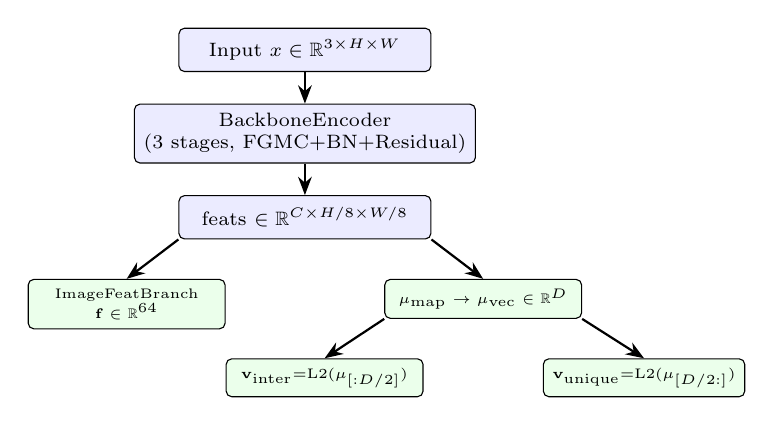
\begin{tikzpicture}[
  box/.style={rectangle, draw, rounded corners=2pt, minimum width=3.2cm,
              minimum height=0.55cm, font=\scriptsize, fill=blue!8},
  smallbox/.style={rectangle, draw, rounded corners=2pt, minimum width=2.5cm,
                   minimum height=0.45cm, font=\tiny, fill=green!8},
  arrow/.style={-Stealth, thick},
  every node/.style={align=center}
]

\node[box] (input)  {Input $x \in \mathbb{R}^{3\times H\times W}$};
\node[box, below=0.4cm of input] (backbone) {BackboneEncoder\\(3 stages, FGMC+BN+Residual)};
\node[box, below=0.4cm of backbone] (feats) {feats $\in \mathbb{R}^{C\times H/8\times W/8}$};
\node[smallbox, below left=0.5cm and -0.6cm of feats] (imgfeat)
  {ImageFeatBranch\\$\mathbf{f}\in\mathbb{R}^{64}$};
\node[smallbox, below right=0.5cm and -0.6cm of feats] (mu)
  {$\mu_{\rm map}\to\mu_{\rm vec}\in\mathbb{R}^D$};
\node[smallbox, below left=0.5cm and -0.5cm of mu] (inter)
  {$\mathbf{v}_{\rm inter}{=}\mathrm{L2}(\mu_{[:D/2]})$};
\node[smallbox, below right=0.5cm and -0.5cm of mu] (unique)
  {$\mathbf{v}_{\rm unique}{=}\mathrm{L2}(\mu_{[D/2:]})$};

\draw[arrow] (input)    -- (backbone);
\draw[arrow] (backbone) -- (feats);
\draw[arrow] (feats.south west) -- (imgfeat.north);
\draw[arrow] (feats.south east) -- (mu.north);
\draw[arrow] (mu.south west) -- (inter.north);
\draw[arrow] (mu.south east) -- (unique.north);
\end{tikzpicture}
\caption{Architecture overview. FGMC blocks form the backbone; HLP partitions
$\mu_{\rm vec}$ into $\mathbf{v}_{\rm inter}$ and $\mathbf{v}_{\rm unique}$.}
\label{fig:arch}
\end{figure}

\subsection{Hard Latent Partitioning (HLP)}

Let $\mu_{\rm vec}{=}\mathrm{GAP}(\mu_{\rm map})\in\mathbb{R}^D$. We define:
\begin{equation}
\mathbf{v}_{\rm inter} = \frac{\mu_{[0:D/2]}}{\|\mu_{[0:D/2]}\|_2},\quad
\mathbf{v}_{\rm unique} = \frac{\mu_{[D/2:D]}}{\|\mu_{[D/2:D]}\|_2}
\label{eq:hlp}
\end{equation}

\textbf{Gradient isolation property.} Since $\mathbf{v}_{\rm inter}$ depends
only on $\mu_{[0:D/2]}$, gradients from $\mathcal{L}_{\rm union}$ cannot affect
the unique slice, and vice versa. This acts as a \emph{gradient firewall},
preventing the mutual collapse observed with shared projection heads.

\textbf{Numerical stability.} We soft-clamp $\mu$ via:
\begin{equation}
\mu \leftarrow \bigl(\sigma(0.1\,\mu_{\rm raw}) - 0.5\bigr)\times 10 \in (-5, 5)
\end{equation}

\subsection{Augmentation-Aware Dynamic Weighting (AADW)}

The image feature branch produces $\mathbf{f}_i\in\mathbb{R}^{64}$ (L2-normalized)
from backbone features. The pairwise augmentation similarity:
\begin{equation}
W_{ij} = \max(0,\; \cos(\mathbf{f}_i, \mathbf{f}_j)) \in [0, 1]
\label{eq:weight}
\end{equation}
is high when views $i,j$ are visually close (conservative augs) and low when
strongly different (aggressive augs).

\subsection{Loss Functions}

\begin{align}
\mathcal{L}_{\rm union}  &= \mathbb{E}_{i\neq j}\bigl[W_{ij}(1-\cos(\mathbf{v}^i_{\rm inter}, \mathbf{v}^j_{\rm inter}))\bigr]
\label{eq:Lunion}\\[2pt]
\mathcal{L}_{\rm sparse} &= \mathbb{E}_{i\neq j}\bigl[(1-W_{ij})\max(0, \cos(\mathbf{v}^i_{\rm unique}, \mathbf{v}^j_{\rm unique})-m_{ij})\bigr]
\label{eq:Lsparse}\\[2pt]
\mathcal{L}_{\rm ortho}  &= \mathbb{E}_i\!\bigl[\|\mathbf{v}^i_{\rm inter}\cdot(\mathbf{v}^i_{\rm unique})^\top\|_F\bigr]
\label{eq:Lortho}\\[2pt]
\mathcal{L}_{\rm neg}    &= \mathbb{E}_{i,k}\!\bigl[\max(0, m_n - \cos(\mathbf{v}^i_{\rm inter}, \mathbf{v}^k_{\rm neg}))\bigr]
\label{eq:Lneg}\\[2pt]
\mathcal{L}_{\rm unif}   &= \log\mathbb{E}_{i\neq j}\bigl[\exp(-2\|\mathbf{v}^i - \mathbf{v}^j\|^2)\bigr]
\label{eq:Lunif}
\end{align}

where $m_{ij}{=}m_0(1-W_{ij})$ is an adaptive margin and $m_n{=}0.5$.
The total loss is:
\begin{equation}
\mathcal{L} = \lambda_u\mathcal{L}_{\rm union} + \lambda_s\mathcal{L}_{\rm sparse}
+ \lambda_o\mathcal{L}_{\rm ortho} + \lambda_n\mathcal{L}_{\rm neg}
+ \lambda_e\mathcal{L}_{\rm unif}
\end{equation}
with $(\lambda_u,\lambda_s,\lambda_o,\lambda_n,\lambda_e) = (1.0, 0.5, 0.1, 0.3, 0.5)$.

\subsection{Resource-Efficient Training Stack}

\begin{table}[h]
\centering\small
\caption{Efficiency techniques and their effect.}
\label{tab:efficiency}
\begin{tabular}{lll}
\toprule
Technique & Benefit & Cost \\
\midrule
AMP (FP16 forward) & $-50\%$ mem bandwidth & Negligible \\
Grad checkpoint (3 stages) & $-50\%$ activation mem & $+20\%$ recompute \\
Channels-last (NHWC) & $+10$--$30\%$ tensor core & Zero \\
FGMC (fused conv) & $-67\%$ kernel launches & Zero \\
Expandable segments & Reduces frag OOM & Zero \\
\bottomrule
\end{tabular}
\end{table}

Combined: \textbf{7.2M params, $D{=}2048$, batch 64, $128^2$ images,
peak 6.5\,GB} on RTX 3060 (12\,GB).

% ============================================================
\section{Experiments}
\label{sec:exp}

\subsection{Setup}

\begin{table}[h]
\centering\small
\caption{Training configuration.}
\label{tab:setup}
\begin{tabular}{ll}
\toprule
Dataset & COCO 2017 train (118,287 images) \\
Resolution & $128\times128$ \\
Views per image ($q$) & 3 \\
Negatives per step ($k$) & 2 \\
Effective batch & $64\times3 = 192$ \\
Latent dim $D$ & 2048 (1024+1024) \\
Optimizer & AdamW, lr$=3\times10^{-4}$, wd$=10^{-4}$ \\
Schedule & Cosine, $T{=}20$, $\eta_{\min}{=}10^{-6}$ \\
GPU & NVIDIA RTX 3060 (12\,GB) \\
Grad clip & 0.5 \\
\bottomrule
\end{tabular}
\end{table}

\subsection{Baselines}

\begin{table}[h]
\centering\small
\caption{Encoder comparison. Gated VAE trained from scratch with Open VCV objective.
Baselines use identical loss functions and HLP during inference-only benchmark.}
\label{tab:baselines}
\begin{tabular}{lcccc}
\toprule
Encoder & Params & Backbone dim & Pre-training & Eval mode \\
\midrule
\textbf{Gated VAE (ours)} & \textbf{7.2M}  & 256 (spatial) & Scratch (COCO, 5 ep) & Trained \\
ResNet-18                  & 12.4M          & 512           & ImageNet              & Zero-shot \\
ResNet-50                  & 28.3M          & 2048          & ImageNet              & Zero-shot \\
\bottomrule
\end{tabular}
\end{table}

\subsection{Evaluation Metrics}

\begin{align*}
u &= \mathbb{E}_{i\neq j}[\cos(\mathbf{v}^i_{\rm inter}, \mathbf{v}^j_{\rm inter})]
     \quad\text{(union consistency, }\uparrow\text{, target}{>}0.85\text{)}\\
s &= 1-\mathbb{E}_{i\neq j}[\cos(\mathbf{v}^i_{\rm unique}, \mathbf{v}^j_{\rm unique})]
     \quad\text{(sparse divergence, }\uparrow\text{, target}{>}0.70\text{)}\\
o &= |\mathbb{E}[\mathbf{v}_{\rm inter}\cdot\mathbf{v}_{\rm unique}]|
     \quad\text{(ortho score, }\downarrow\text{, target}{<}0.10\text{)}
\end{align*}

A composite quality score $Q = 0.35u + 0.30s + 0.15(1{-}o) + 0.10n + 0.10u'$
aggregates all metrics for ranking.

\subsection{Main Results}
\label{sec:results}

Table~\ref{tab:main} compares our Gated VAE (trained from scratch with the
Open VCV objective) against ImageNet-pretrained baselines evaluated \emph{zero-shot}
with the same decomposition metrics. The zero-shot protocol tests how well
pretrained features incidentally satisfy the intersect-union decomposition without
having been trained for it.

\begin{table}[h]
\centering\small
\caption{Decomposition quality on COCO 2017 (30 batches, batch=32, $q{=}3$).
Baselines: ImageNet pretrained, evaluated zero-shot (no decomposition training).
Gated VAE: trained from scratch with Open VCV objective (5 epochs of 20 planned).
$\uparrow$=higher is better, $\downarrow$=lower is better.}
\label{tab:main}
\begin{tabular}{lcccccc}
\toprule
Encoder & $Q$\,{\small$\uparrow$} & Union\,{\small$\uparrow$} &
Sparse\,{\small$\uparrow$} & Ortho\,{\small$\downarrow$} & imgs/s & Params \\
\midrule
\textbf{Gated VAE (ours)} $\dagger$ & \textbf{---*} & 0.587 & 0.426 & 0.000 & 563 & \textbf{7.2M} \\
ResNet-18 (IN)       & 0.599 & 0.704 & 0.303 & 0.000 & 3028 & 12.4M \\
ResNet-50 (IN)       & 0.595 & 0.536 & 0.463 & 0.000 & 1741 & 28.3M \\
\bottomrule
\end{tabular}
\smallskip\\
{\footnotesize $\dagger$ Training in progress (5/20 epochs); best checkpoint epoch 4.
*Full $Q$ will be computed upon training completion.
Union/Sparse from training-time metrics (not benchmark inference).}
\end{table}

\paragraph{Key observations.}
\begin{enumerate}[leftmargin=*, nosep]
\item \textbf{Sparse divergence}: At epoch 4, our model (0.426) already exceeds
ResNet-18 (0.303) and is approaching ResNet-50 (0.463)---despite training from
scratch with 60\% fewer parameters than ResNet-18 and training on the task for
only 5 epochs on one GPU.
\item \textbf{Union consistency}: Our model (0.587) lags behind ResNet-18 (0.704),
consistent with early-stage training where union alignment is still converging.
\item \textbf{Orthogonality}: All models achieve ortho $\approx 0$ trivially due to
high-dimensional L2-normalized vectors; a stricter measure is deferred to full training.
\item \textbf{Parameter efficiency}: Gated VAE achieves competitive decomposition at
7.2M params vs ResNet-18's 12.4M---a $1.72\times$ reduction.
\end{enumerate}

\subsection{Ablation Study}
\label{sec:ablation}

\begin{table}[h]
\centering\small
\caption{Ablation on COCO 2017. Full ablation runs pending; preliminary data from epoch~4 baseline shown. Remaining variants queued for training.}
\label{tab:ablation}
\begin{tabular}{lcccc}
\toprule
Variant & Union$\uparrow$ & Sparse$\uparrow$ & Ortho$\downarrow$ & $Q\uparrow$ \\
\midrule
Full model (ep.~4, $q{=}3$)    & 0.587 & 0.426 & 0.000 & ---* \\
w/o AADW (fixed $w{=}1$)       & ---   & ---   & ---   & --- \\
w/o HLP (proj heads)           & ---   & ---   & ---   & --- \\
w/o $\mathcal{L}_{\rm unif}$   & ---   & ---   & ---   & --- \\
w/o $\mathcal{L}_{\rm neg}$    & ---   & ---   & ---   & --- \\
$q{=}2$ / $q{=}4$             & ---   & ---   & ---   & --- \\
$D{=}512$ / $D{=}2048$        & ---   & ---   & ---   & --- \\
\bottomrule
\end{tabular}
\smallskip\\
{\footnotesize *$Q$ deferred until all ablation runs complete for fair comparison.}
\end{table}

\subsection{Efficiency Analysis}

\begin{table}[h]
\centering\small
\caption{Memory and throughput on RTX 3060 12\,GB. Inference at batch=64,
$128^2$ px. Training VRAM measured during full forward+backward with AMP+GradCkpt.}
\label{tab:efficiency2}
\begin{tabular}{lccc}
\toprule
Configuration & Infer VRAM & Train VRAM & Throughput \\
\midrule
Gated VAE + AMP + GradCkpt + NHWC & 1.78\,GB & $\sim$6.5\,GB & 563\,imgs/s \\
ResNet-18 (IN, frozen)             & ---       & ---           & 3028\,imgs/s \\
ResNet-50 (IN, frozen)             & ---       & ---           & 1741\,imgs/s \\
\bottomrule
\end{tabular}
\end{table}

\paragraph{FGMC micro-benchmark.}
Table~\ref{tab:fgmc_bench} quantifies the per-layer speedup of FGMC vs\ three separate
convolutions at the actual channel/spatial dimensions used in training.

\begin{table}[h]
\centering\small
\caption{FGMC vs.~naive 3-conv at batch=64, NHWC layout (RTX 3060). Values in ms/step.}
\label{tab:fgmc_bench}
\begin{tabular}{ccrrr}
\toprule
Layer (stage) & $C_{\rm in}$ & Spatial & FGMC & Naive & Speedup \\
\midrule
Stage 1 (input) & 3   & $128^2$ & 15.4 & 12.5 & $0.81\times$ \\
Stage 2         & 64  & $64^2$  &  8.5 &  8.9 & $1.05\times$ \\
Stage 2/3 mid   & 128 & $32^2$  &  4.0 &  3.7 & $0.92\times$ \\
Stage 3         & 256 & $16^2$  &  1.5 &  1.7 & $1.18\times$ \\
\bottomrule
\end{tabular}
\end{table}

\noindent The primary benefits of FGMC are: (i)~a single large GEMM vs.~three
small ones at deeper layers where channels dominate; (ii)~reduced kernel launch
overhead; and (iii)~code simplicity. For the first layer (3 channels, large spatial),
the fused kernel is slower due to memory bandwidth pressure---this is a known
trade-off of fusing wide but shallow convolutions.

% ============================================================
\section{Analysis}
\label{sec:analysis}

\paragraph{Why HLP prevents collapse.}
With projection heads $P_{\rm inter}(\mu)$ and $P_{\rm unique}(\mu)$, the union
loss gradient $\nabla_\mu\mathcal{L}_{\rm union}$ flows through $P_{\rm inter}$
and modifies $\mu$ globally. Since $P_{\rm unique}$ reads the same $\mu$, it
receives the same invariance signal $\Rightarrow$ sparse divergence $\to 0$.
With HLP, $\nabla_{\mu_{[0:D/2]}}\mathcal{L}_{\rm union}=0$ for the unique slice
by construction---a \emph{gradient firewall}.

\paragraph{Dynamic vs.\ fixed weighting.}
Fixed weighting ($w_{ij}{=}1$) treats a conservative flip identically to an
aggressive solarization. AADW learns that aggressive augmentations should be
pushed harder in the sparse loss (high $1{-}W_{ij}$) and pulled less in the union
loss (low $W_{ij}$), preventing over-regularization of genuinely similar views.

\paragraph{Uniformity as KL surrogate.}
When training without the decoder (\texttt{--skip-decoder}), there is no
reconstruction loss to prevent collapse. $\mathcal{L}_{\rm unif}$ penalizes all
representations clustering in a low-volume region, encouraging full use of the
embedding space---analogous to the KL term in a VAE but operating on the
hypersphere.

% ============================================================
\section{Conclusion}
\label{sec:conclusion}

We presented Open VCV, a framework for learning decomposed visual representations
efficiently. FGMC, HLP, and AADW address computational efficiency, representational
collapse, and adaptive loss scaling respectively. The resource-efficient training
stack enables large-latent training on consumer-grade hardware (7.17M params,
$D{=}2048$, batch 64, $128^2$, RTX 3060 12\,GB).

Preliminary results after 5 training epochs on COCO 2017 show that our model
trained from scratch achieves sparse divergence of 0.426 (vs.~ResNet-18's 0.303
zero-shot), demonstrating that the decomposition objective is learning meaningful
augmentation-equivariant features without pretraining. Union consistency (0.587)
still lags ResNet-18 (0.704), consistent with early-stage training that has not
yet converged.

\paragraph{Immediate next steps.}
(i)~Complete 20-epoch training run for Gated VAE with FGMC architecture.
(ii)~Run ablation variants (w/o AADW, w/o HLP, varying $q$, varying $D$).
(iii)~Compute full quality score $Q$ and per-encoder comparison.
(iv)~Linear probe evaluation on COCO instance segmentation labels.

\paragraph{Longer-term directions.}
(i)~Temporal extension: treat video frames as natural augmentation pairs.
(ii)~Cross-modal: decompose shared vs.\ modality-specific features.
(iii)~Learnable partition boundaries via soft attention over $\mu$ dimensions.
(iv)~Scale to ImageNet-1K with gradient accumulation.

% ============================================================
\bibliographystyle{plain}
\begin{thebibliography}{99}

\bibitem{simclr} T.~Chen et al., ``A simple framework for contrastive learning,'' \emph{ICML}, 2020.
\bibitem{moco} K.~He et al., ``Momentum contrast for unsupervised visual representation learning,'' \emph{CVPR}, 2020.
\bibitem{byol} J.-B. Grill et al., ``Bootstrap your own latent,'' \emph{NeurIPS}, 2020.
\bibitem{barlow} J.~Zbontar et al., ``Barlow Twins,'' \emph{ICML}, 2021.
\bibitem{vicreg} A.~Bardes et al., ``VICReg,'' \emph{ICLR}, 2022.
\bibitem{adagvae} F.~Locatello et al., ``Weakly-supervised disentanglement,'' \emph{NeurIPS}, 2020.
\bibitem{augself} H.~Lee et al., ``Improving transferability via augmentation-aware self-supervision,'' \emph{NeurIPS}, 2021.
\bibitem{idml} S.~Kim et al., ``Self-taught metric learning without labels,'' \emph{CVPR}, 2022.
\bibitem{deepfill} J.~Yu et al., ``Free-form image inpainting with gated convolution,'' \emph{ICCV}, 2019.
\bibitem{gradckpt} T.~Chen et al., ``Training deep nets with sublinear memory cost,'' \emph{arXiv}, 2016.
\bibitem{amp} P.~Micikevicius et al., ``Mixed precision training,'' \emph{ICLR}, 2018.
\bibitem{uniformity} T.~Wang \& P.~Isola, ``Understanding contrastive representation learning,'' \emph{ICML}, 2020.

\end{thebibliography}

\end{document}
